\documentclass{scrartcl}
\usepackage[utf8]{inputenc}
\usepackage[T1]{fontenc}

\usepackage[margin=2.5cm]{geometry}
\usepackage[english]{babel}
\usepackage[dvipsnames,usenames]{xcolor}
\usepackage[colorlinks=true,linkcolor=Blue,citecolor=ForestGreen]{hyperref} 
\usepackage{xspace}
\usepackage[style=alphabetic]{biblatex}
\usepackage{bm}
\usepackage{newpxtext, eulerpx}
\usepackage{epigraph}
\usepackage{etoolbox}
\usepackage{multicol}
\usepackage{graphicx}
\usepackage{wrapfig}
\usepackage{microtype}
\usepackage{listings}
\usepackage{xifthen}
\usepackage{mwe}
\usepackage{subcaption}
\usepackage{float}
\usepackage{booktabs}
\usepackage{tabularx}
\usepackage{algorithm}
\usepackage{algpseudocodex}

\setlength{\columnsep}{0,1cm}

\addbibresource{sources.bib}

% Allow usage of " for quotes
\usepackage{csquotes}
\MakeOuterQuote{"}

\newif\ifdraft
\draftfalse

\lstset{
  basicstyle=\footnotesize\ttfamily,breaklines=true,mathescape=true,
  columns=fullflexible, frame=single,
  postbreak=\mbox{\textcolor{red}{$\hookrightarrow$}\space},
  language=[Sharp]C,
  numbers=left,showstringspaces=false
}

% LaTeX-Vorlage teilweise übernommen von https://komascript.de/node/2184

\newcommand{\zB}{z.\,B.\xspace}
\newcommand{\TODO}[1]{\textbf{\textcolor{red}{\ifthenelse{\isempty{#1}}{TODO!}{TODO: #1}}}\xspace}
\newcommand{\SEE}{\textsc{SEE}}
\newcommand{\code}[1]{\TODO{Use lstinline here!}}
\newcommand{\web}[2]{\url{#1} \textit{(last access: #2)}}

\DeclareMathOperator*{\argmin}{arg\,min}

% Andere Font für Beschriftungen
\setkomafont{caption}{\footnotesize\itshape}
\setkomafont{captionlabel}{\usekomafont{caption}}

% Mehr Abstande für wrapfig
\setlength{\columnsep}{12pt}

\begin{document}
% ----------------------------------------------------------------------------
\title{
  Building Code Cities using \mbox{the Language Server Protocol}
  \ifdraft
    -- \emph{DRAFT} --
  \fi
}
\subtitle{Exposé}
\author{Falko Galperin}
\date{\today} 

\maketitle

% ----------------------------------------------------------------------------
% Inhaltsverzeichnis:
\begingroup
  \tableofcontents
\endgroup
\newpage
% ----------------------------------------------------------------------------

\section{Motivation}
Visualization in general often helps facilitate the understanding of complex systems by representing them with a simplified visual model.
This can be especially helpful in the area of software engineering, where it is often hard to get an intuitive overview of large software systems.
One such software visualization---called \SEE{}---is being developed at the University of Bremen and will be introduced in the next section.


\subsection{SEE}
\SEE{} (\emph{Software Engineering Experience}) is an interactive software visualization tool using the code city metaphor in 3D, developed in the {Unity} game engine.
It features collaborative "multiplayer" functionality across multiple platforms\footnote{
  Notably, besides usual desktop and touchscreen-based environments, virtual reality (e.g., via the \emph{Valve Index}) is supported as well.
}, allowing multiple participants to view and interact with the same code city together.

\begin{wrapfigure}[24]{R}{0.6\textwidth}
    \centering
    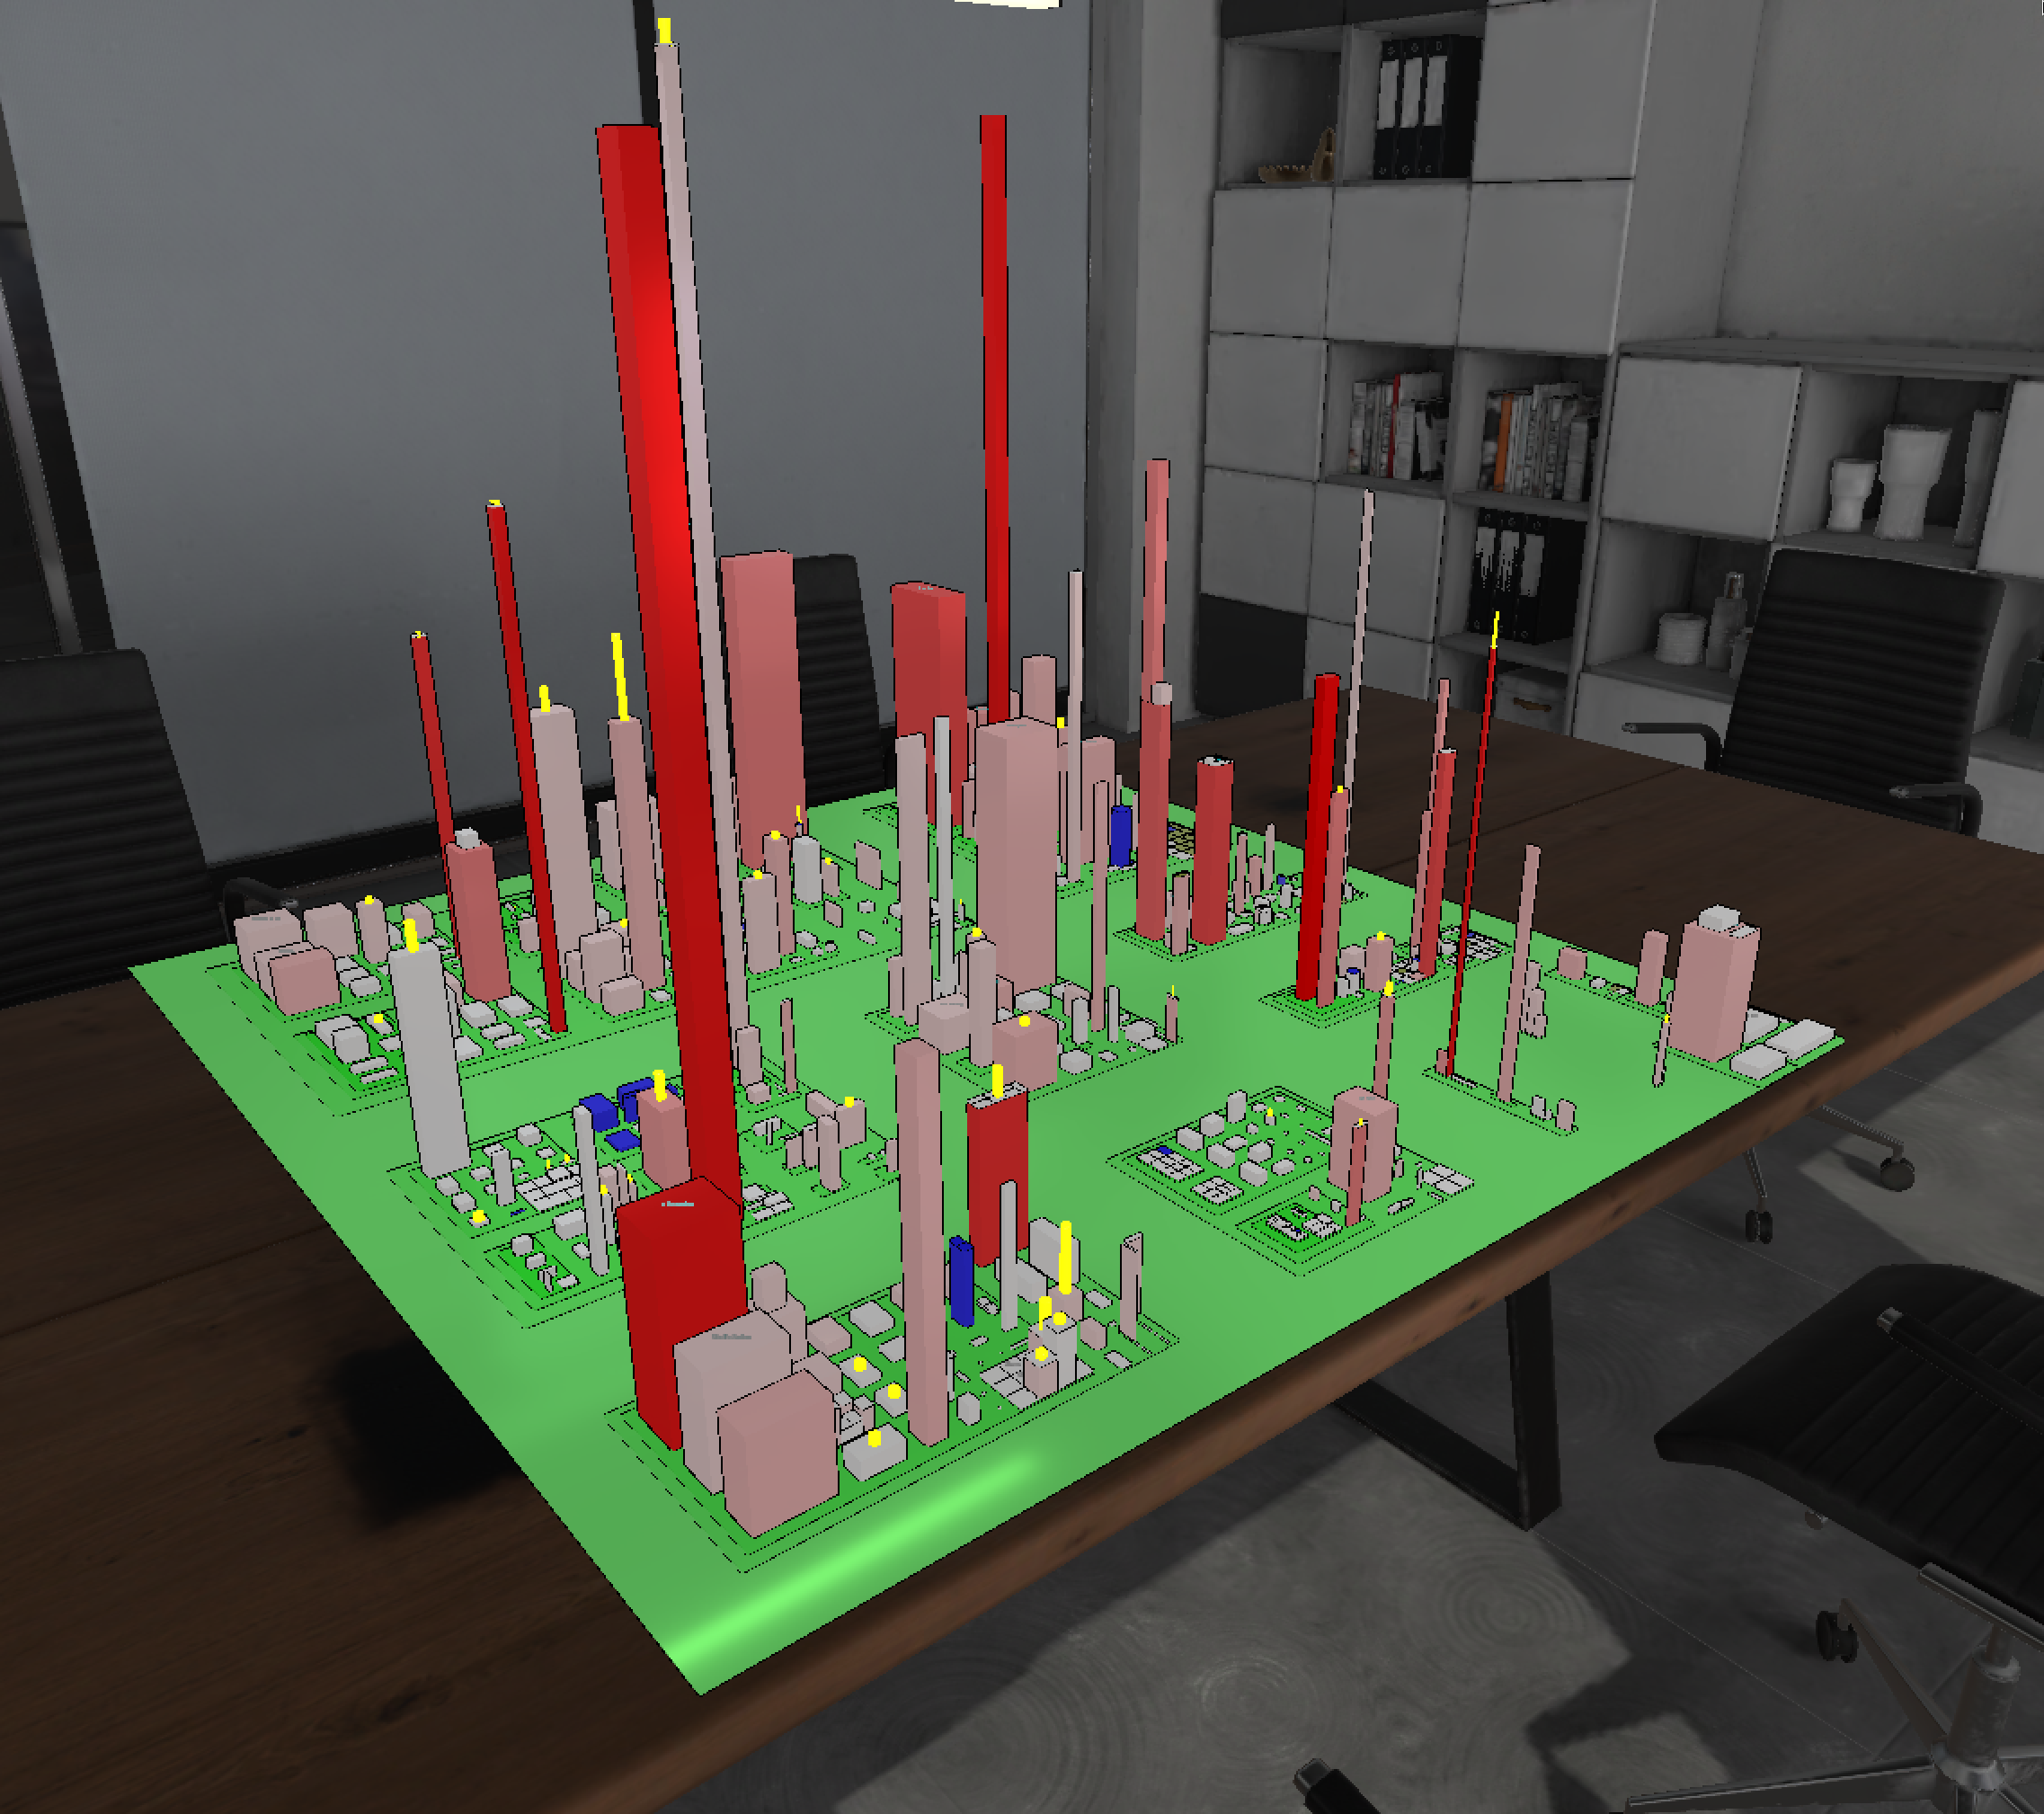
\includegraphics[width=0.6\textwidth]{figures/SEE_city}
    \caption{An example of a code city visualized in \SEE{}.}\label{fig:city}
\end{wrapfigure}

In the code city metaphor, software components are visualized as buildings within a city.
Various metrics from the original software can then be represented by different visual properties of each building---for example, the lines of code within a file might correlate to the height of the corresponding building.
Relationships\footnote{
  The exception to this are part-of relations, that is, which component belongs to which other component.
  These are instead visualized in \SEE{} by buildings being nested within their corresponding "parent" building.
} between software components, such as where components are referenced, are instead represented by edges drawn between the respective buildings.
In this way, the data model of \SEE{} can be represented as a graph in which the software components are the nodes and the relationships are the edges.

\begin{figure}
  \begin{center}
    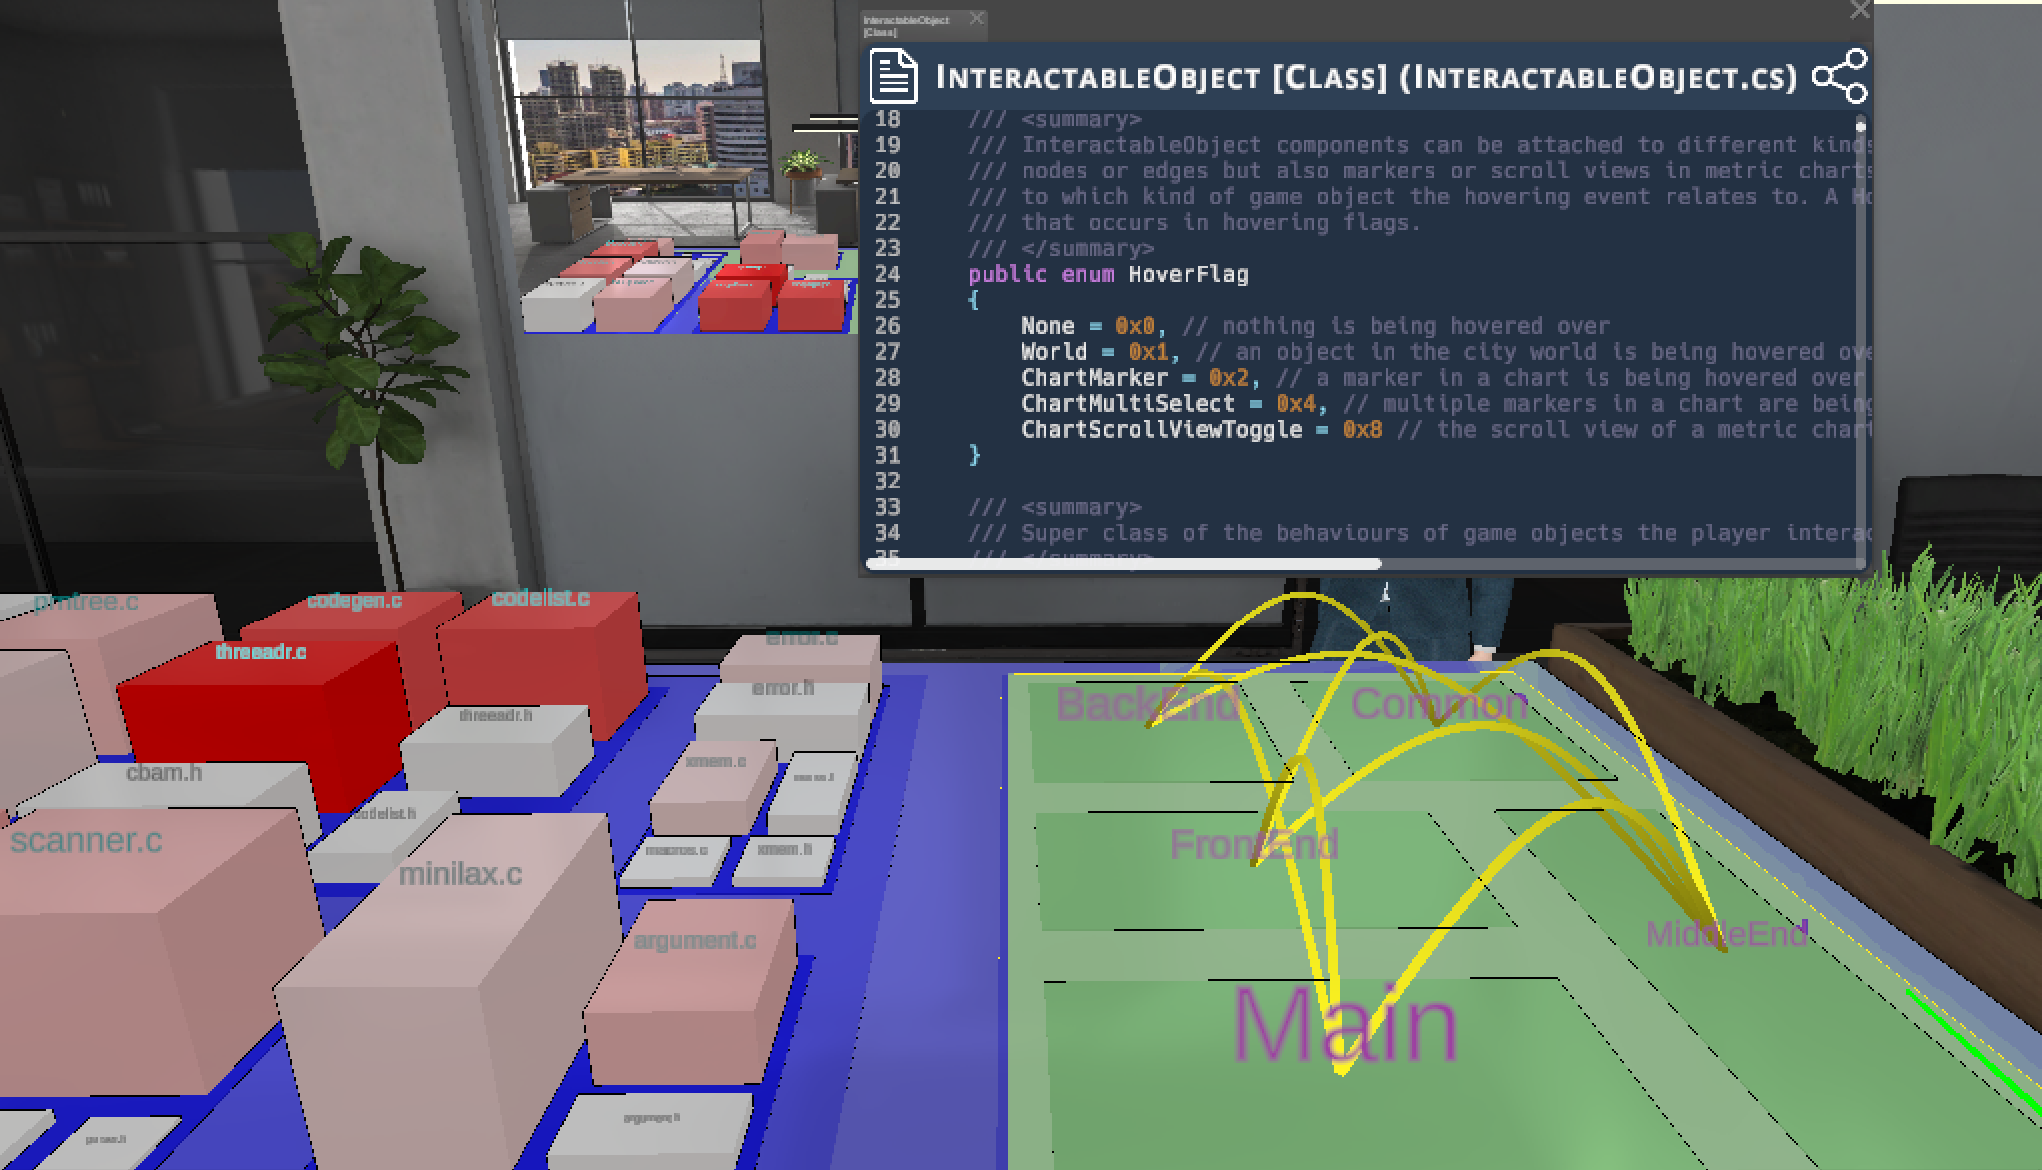
\includegraphics[width=0.75\textwidth,trim={35cm 0 0 20cm},clip]{figures/SEE_readme}
  \end{center}
  \caption{An example of what edges can look like in \SEE{}.}\label{fig:edges}
\end{figure}


For example, in \autoref{fig:city}, we can see the source code of \SEE{} itself rendered as a code city.
A few very tall buildings---indicating that the respective component is very big and that a refactoring into smaller pieces may be in order---immediately jump out.
Additionally, this visualization also makes the relative cyclomatic complexity~\cite{mccabe} readily apparent:
the redder a node, the higher its cyclomatic complexity.
\autoref{fig:edges} instead visualizes the modeled architecture of a very small system, as compared to a city "empirically" generated by an implementation like in the previous example.
Here, we can also see yellow edges between the components, in this case representing desired references that should be present between components.

Currently, code cities in \SEE{} are rendered by reading in pre-made GXL files, which can be created by the proprietary Axivion Suite.
This approach has the disadvantage of only supporting languages supported by the Axivion Suite, as well as making regenerating cities (e.g., if the source code changed) fairly cumbersome.
Another current shortcoming of \SEE{} is that information about the source code available to the user is limited when compared to an IDE---for example, quickly displaying documentation for a given component by hovering over it is not supported.
This is where the Language Server Protocol can help.

\subsection{Language Server Protocol}

As stated on its website:
\begin{displayquote}[\cite{lsp}]
  Adding features like auto complete, go to definition, or documentation on hover for a programming language takes significant effort. Traditionally[,] this work had to be repeated for each development tool, as each tool provides different APIs for implementing the same feature.

A Language Server is meant to provide the language-specific smarts and communicate with development tools over a protocol that enables inter-process communication.

The idea behind the Language Server Protocol (LSP) is to standardize the protocol for how such servers and development tools communicate. This way, a single Language Server can be re-used in multiple development tools, which in turn can support multiple languages with minimal effort.
\end{displayquote}

\begin{figure}
  \begin{center}
    \subcaptionbox{IDE development without LSP.\label{fig:lspwithout}}{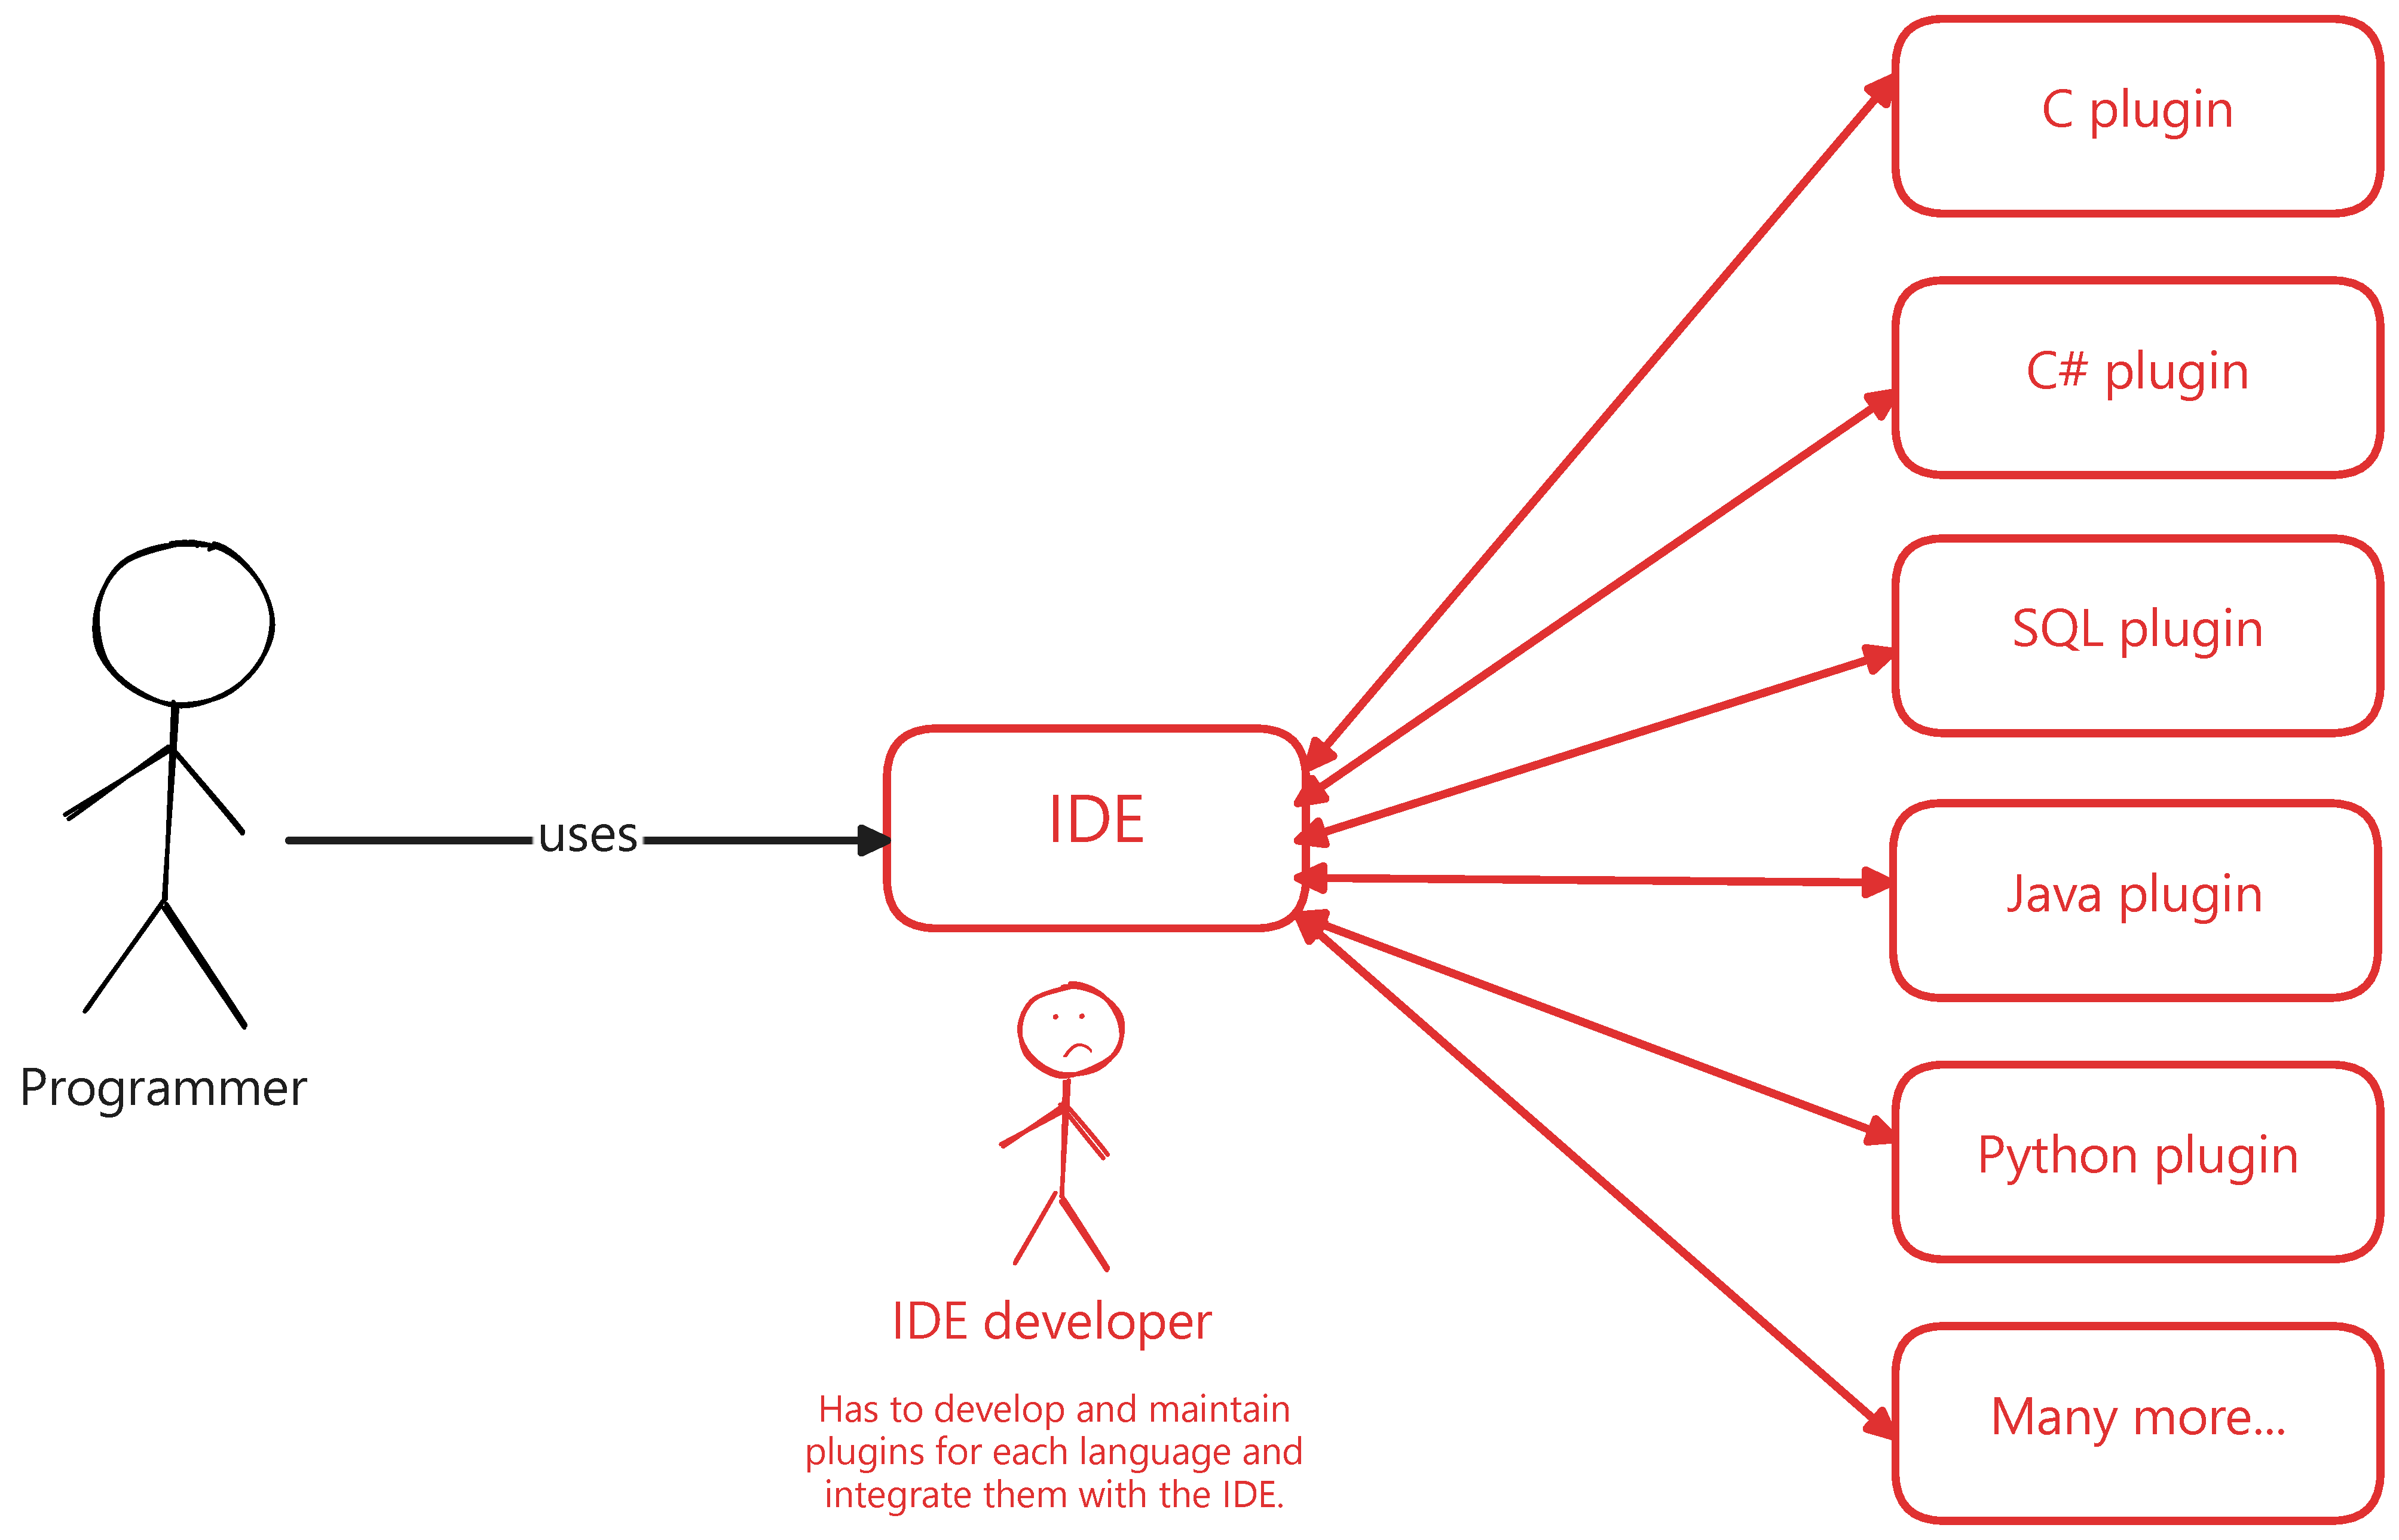
\includegraphics[width=0.95\textwidth]{figures/overview_lsp_without_lsp}}
    \subcaptionbox{IDE development with LSP.\label{fig:lspwith}}{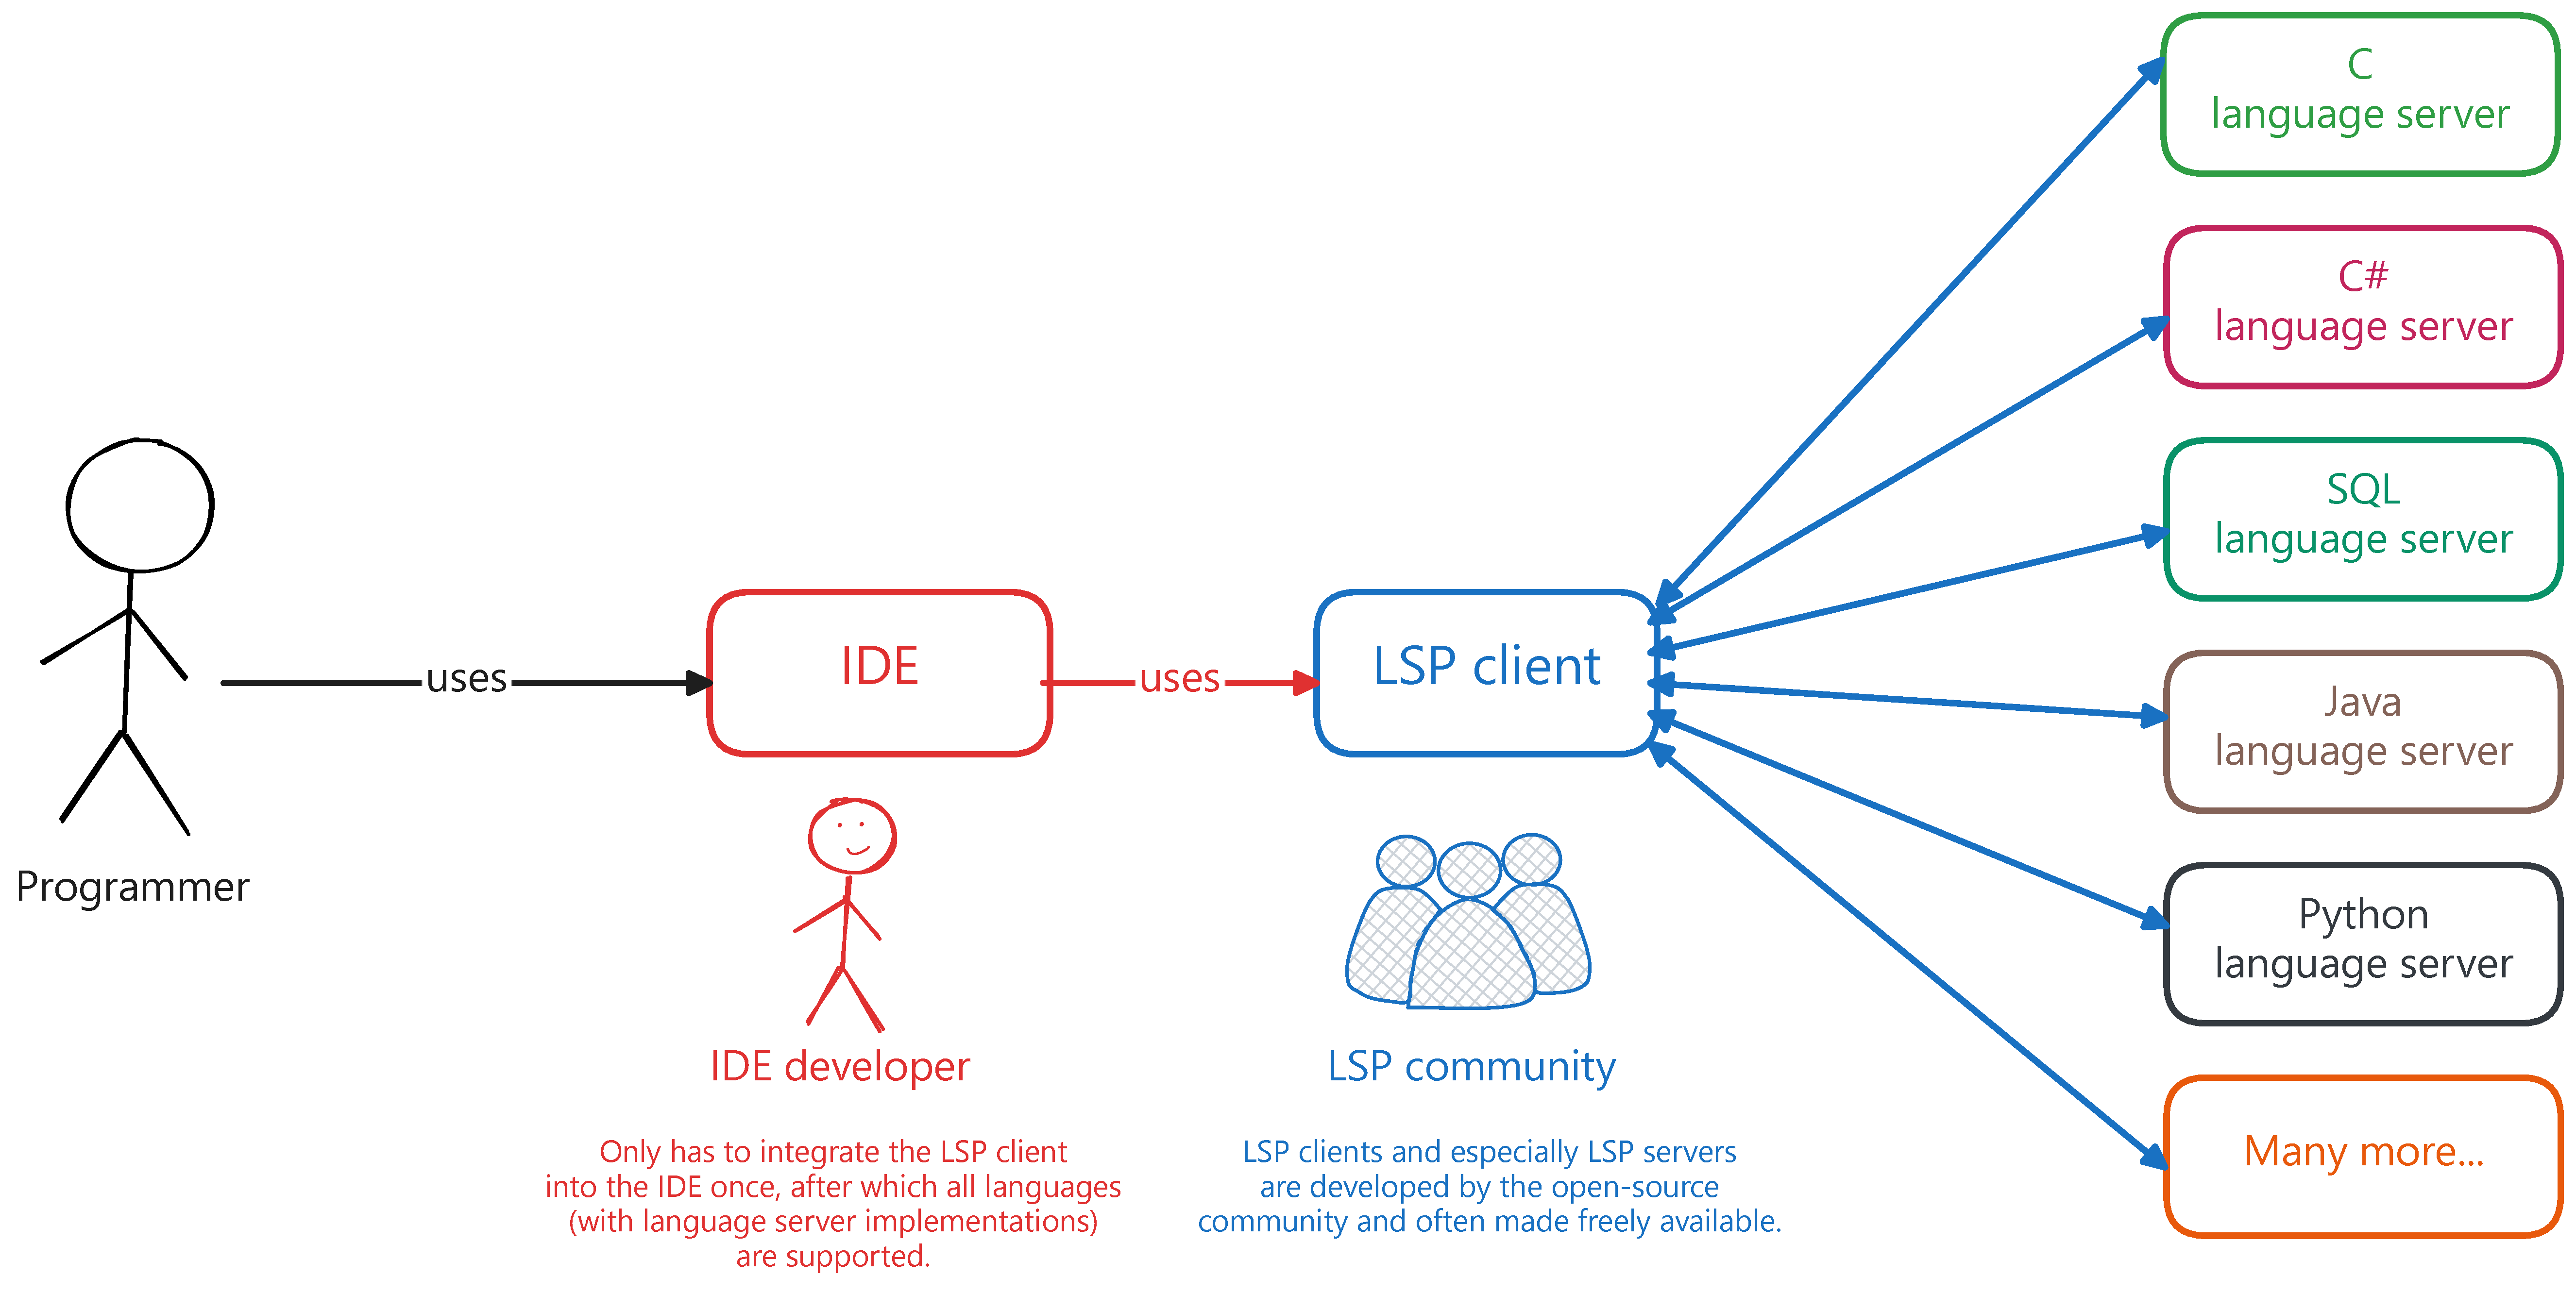
\includegraphics[width=0.95\textwidth]{figures/overview_lsp_with_lsp}}
  \end{center}
  \caption{An illustration of how LSP can help simplify IDE development.}\label{fig:lsp}
\end{figure}

\noindent{}As LSP is a central component of my master's thesis, I have created a diagram in \autoref{fig:lsp} in the hopes to strengthen intuitions around the use of the protocol.
While the LSP specification has originally been created by Microsoft, it is by now an open-source project\footnote{
  Available at \web{https://github.com/Microsoft/language-server-protocol}{2024-01-28}.
}, where changes can be actively proposed using issues or pull requests.
Apart from the specification itself, a great number of open-source implementations of language servers for all kinds of programming languages from Ada to Zig exist.
A partial overview of available implementations is listed at \web{https://microsoft.github.io/language-server-protocol/implementors/servers/}{2024-01-29}.

The protocol introduces the concept of so-called \emph{capabilities}, which define a specific set of features a given language server (and language client) support.
These include navigational features, like the ability to jump to a variable's declaration, and editing-related features, such as autocomplete.
To give a specific example of what an LSP capability might look like in practice, the \texttt{texlab}\footnote{
  \web{https://github.com/latex-lsp/texlab}{2024-01-28}
} language server for \LaTeX{}---which I am using while authoring this very document---provides a list of available packages when one starts typing text after "\lstinline[language={[LaTeX]TeX}]+\usepackage{+".
Additionally, for the currently hovered package, a short description of it is displayed.
A screenshot of this behavior within the \textsc{Neovim} editor is provided in \autoref{fig:mwe}.

\begin{figure}
  \begin{center}
    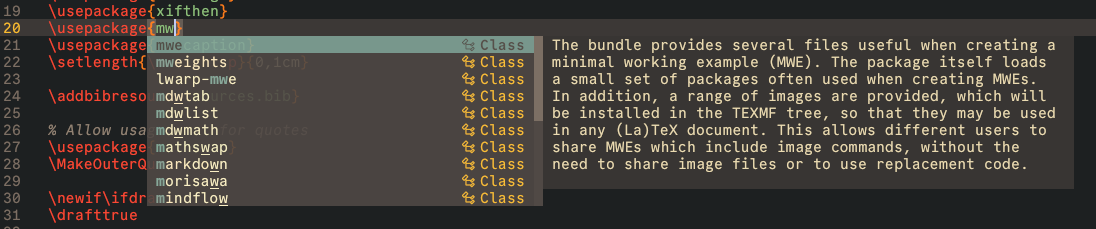
\includegraphics[width=0.95\textwidth]{figures/mwe}
  \end{center}
  \caption{An example of the \texttt{texlab} Language Server running in \textsc{Neovim} (on this exposé).}\label{fig:mwe}
\end{figure}

The counterparts to Language Servers are the Language Clients:
These are the IDEs and editors that incorporate the language server into themselves.
Examples for IDEs that support acting as a Language Client in the LSP context include \emph{Eclipse, Emacs, IntelliJ IDEA} (including other JetBrains IDEs), \emph{(Neo)vim}, and \emph{Visual Studio}.

\section{Goals}\label{sec:goals}
The goal of this master's thesis is to integrate the Language Server Protocol into \SEE{} by making it a Language Client, then evaluate this implementation by comparing it with traditional IDEs in a user study.
To this end, the main contribution will be a way of generating code cities using the Language Server, where all the information obtainable by relevant LSP capabilities should be manifested\footnote{
  Since there is a lot of diverse data available via LSP, it makes sense to only immediately display the most pertinent information and make the rest of it available upon request within \SEE{}'s UI.
} in the city in a suitable way.
This is an unintended (or at the very least, unusual) use of LSP and may require some experimentation.

\begin{wrapfigure}{L}{0.6\textwidth}
    \centering
    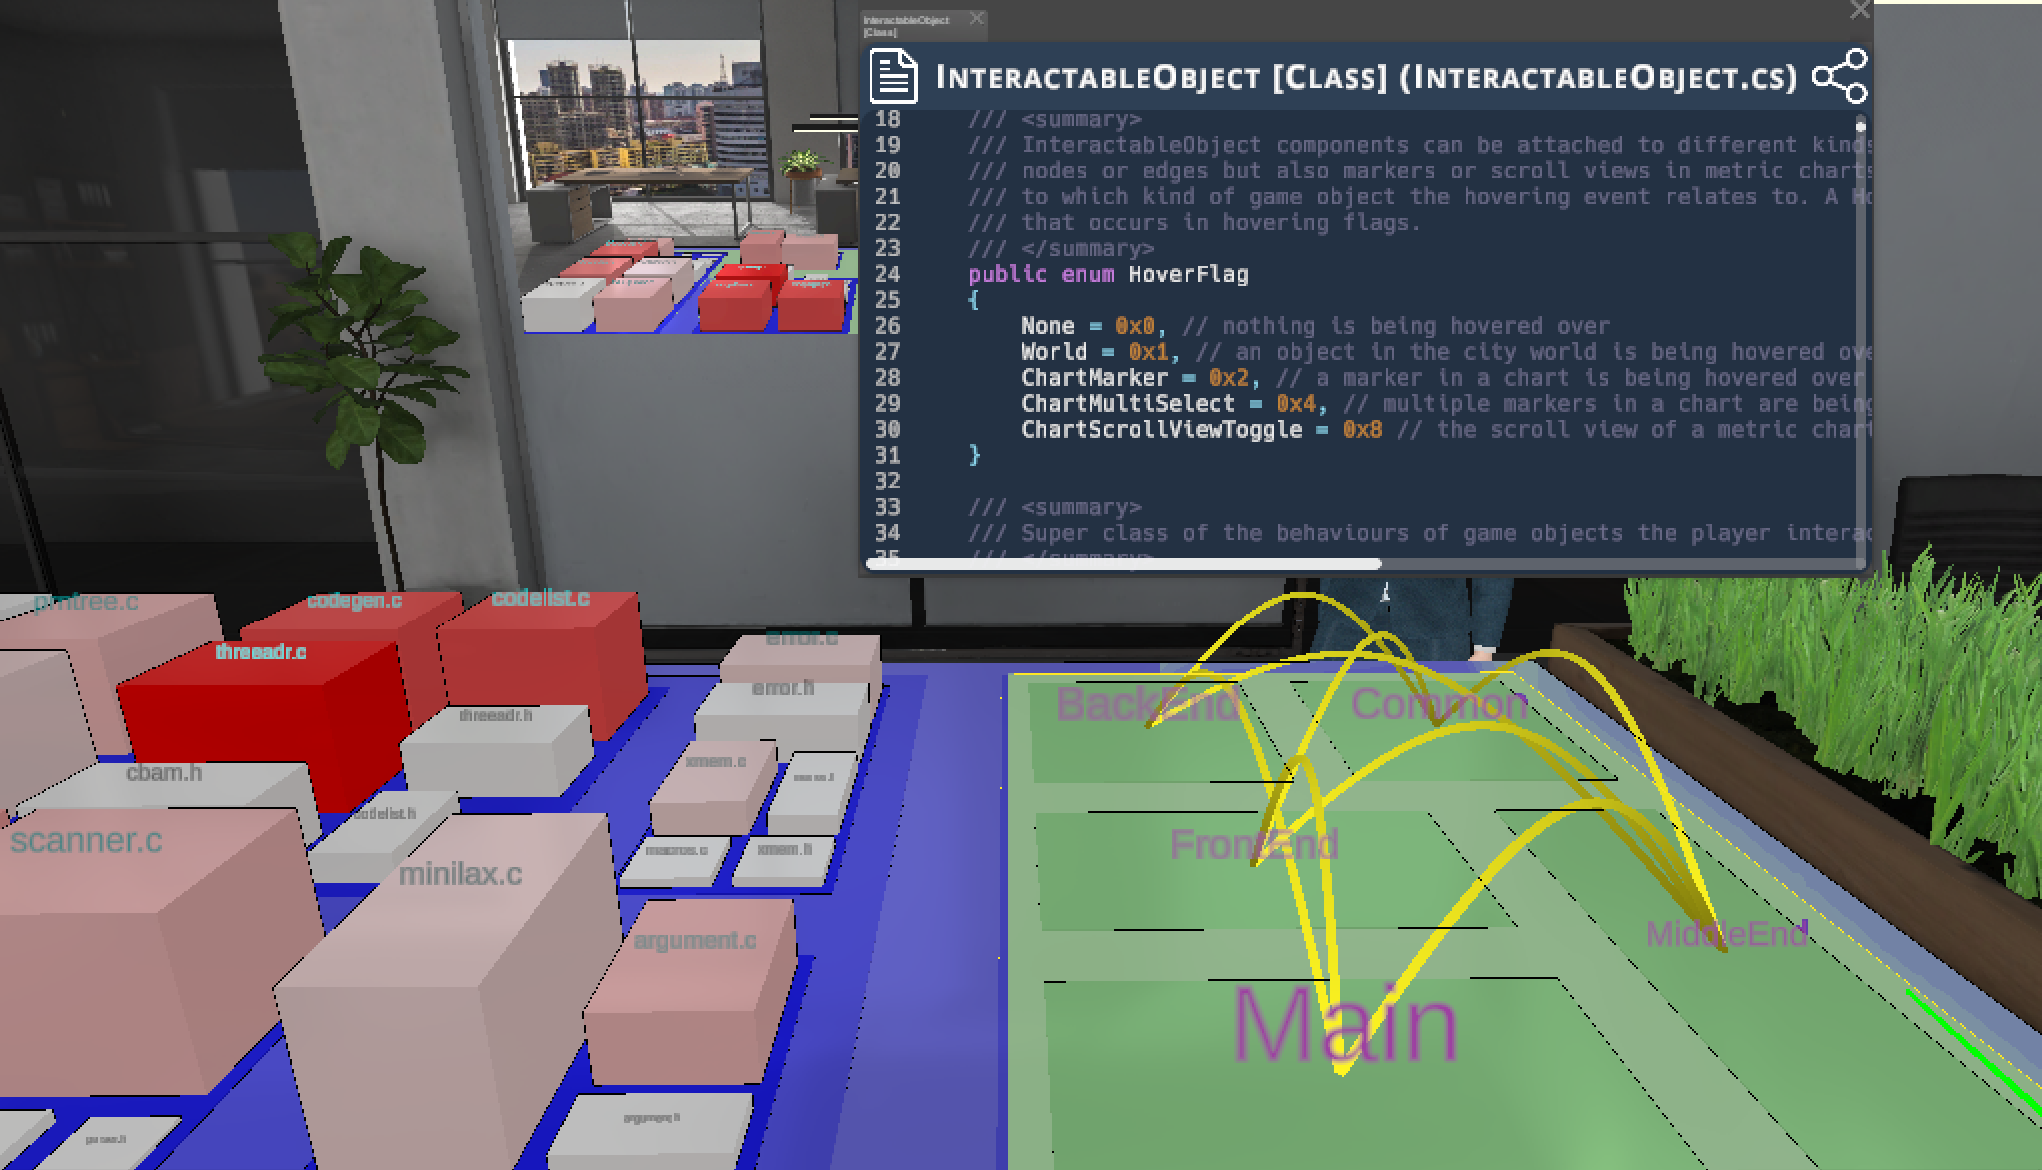
\includegraphics[width=0.6\textwidth,trim={30.5cm 22cm 6cm 0},clip]{figures/SEE_readme}
    \caption{A code window.}\label{fig:window}
\end{wrapfigure}

Apart from the code cities, \SEE{} also provides the so-called \emph{code windows}, in which the source code of a specific component can be viewed in a similar way as in an IDE.
This can be seen in \autoref{fig:window}.
An additional goal of this master's thesis is to enhance the functionality of the code windows by implementing more IDE-like behavior into it (e.g., allowing users to go to a variable's declaration, or displaying diagnostics inline) using the Language Server.

It should be noted that any LSP capabilities which involve modifying the underlying software project is out of scope for this master's thesis.
Rewriting the code windows to be editable (in a way that distributes the edits over the network) is complex enough to warrant its own thesis~\cite[see also][]{moritz}, not even taking into account that this would also more than double the number of LSP capabilities that would then become useful to implement.
As such, only LSP capabilities that are "read-only" (i.e., do not modify the source code or project structure in any way) will be considered when planning which features to implement as part of the thesis.
Consult \autoref{sec:capabilities} for a full list of LSP capabilities which I plan to implement.

Additionally, I will not implement the C\# interface to the Language Server Protocol (i.e., translating between C\# method calls and JSON-RPC calls).
There already exist well-made interfaces for this purpose\footnote{
  Such as OmniSharp's implementation of LSP in C\#, which I plan to use:
  \web{https://github.com/OmniSharp/csharp-language-server-protocol}{2024-28-01}
}, and the focus of the thesis will be on the integration of the protocol's \emph{data} into \SEE{}'s code cities and code windows, not the integration of the protocol itself.

\subsection{Mandatory goals}
In short, I plan to fulfill all of the following goals as part of this thesis:
\begin{itemize}
  \item Integrating an LSP SDK into \SEE{} and allowing users to manage Language Servers from within SEE
  \item Making \SEE{} an LSP Language Client, such that:
    \begin{enumerate}
      \item Code cities can be generated directly from source code directories, using Language Servers that \SEE{} interfaces with,
      \item Code windows gain "read-only" IDE-like functionality, covering behavior of capabilities listed in \autoref{sec:capabilities}, and
      \item Code cities gain similar functionality (where applicable), such as displaying relevant documentation when hovering over a node.
    \end{enumerate}
  \item Evaluating the above empirically via a user study.
\end{itemize}

\subsection{Further goals}
These are ideas for further goals, which probably won't be implemented as part of the master's thesis, but build on the parts described above and introduce additional features.
\begin{itemize}
  \item Regenerating a code city automatically when the underlying source code is modified
  \item Offering to download and install Language Servers from within \SEE{}
  \item Introducing LSP-assisted edit functionalities for both code cities and code windows
  \item Using the Language Server Index Format~\cite{lsif} to build code cities for remote projects (e.g., ones hosted in remote Git repositories)
  \item Supporting additional LSP capabilities not included in \autoref{sec:capabilities}, such as folding ranges or inlay hints
  \item Integrating \SEE{}'s LSP implementation with the Debug Adapter Protocol~\cite{dap} (e.g., to provide inline values in debugging contexts)
  \item Implementing a Language Server for the Axivion Suite
\end{itemize}

\section{Approach}
In this section, I will describe how to fulfill the above goals in terms of the implementation and subsequent evaluation.

\subsection{Implementation}\label{subsec:implementation}

As outlined in \autoref{sec:goals}, the implementation can be divided into three parts:
\nameref{subsubsec:generate}, \nameref{subsubsec:window}, and \nameref{subsubsec:city}.
A general visualization of the approach and the concrete changes in \SEE{} for the implementation is given in \autoref{fig:seeplan}.

\begin{figure}
  \begin{center}
    \subcaptionbox{\SEE{} as it exists right now. The analyzers on the right are developed by Axivion.}{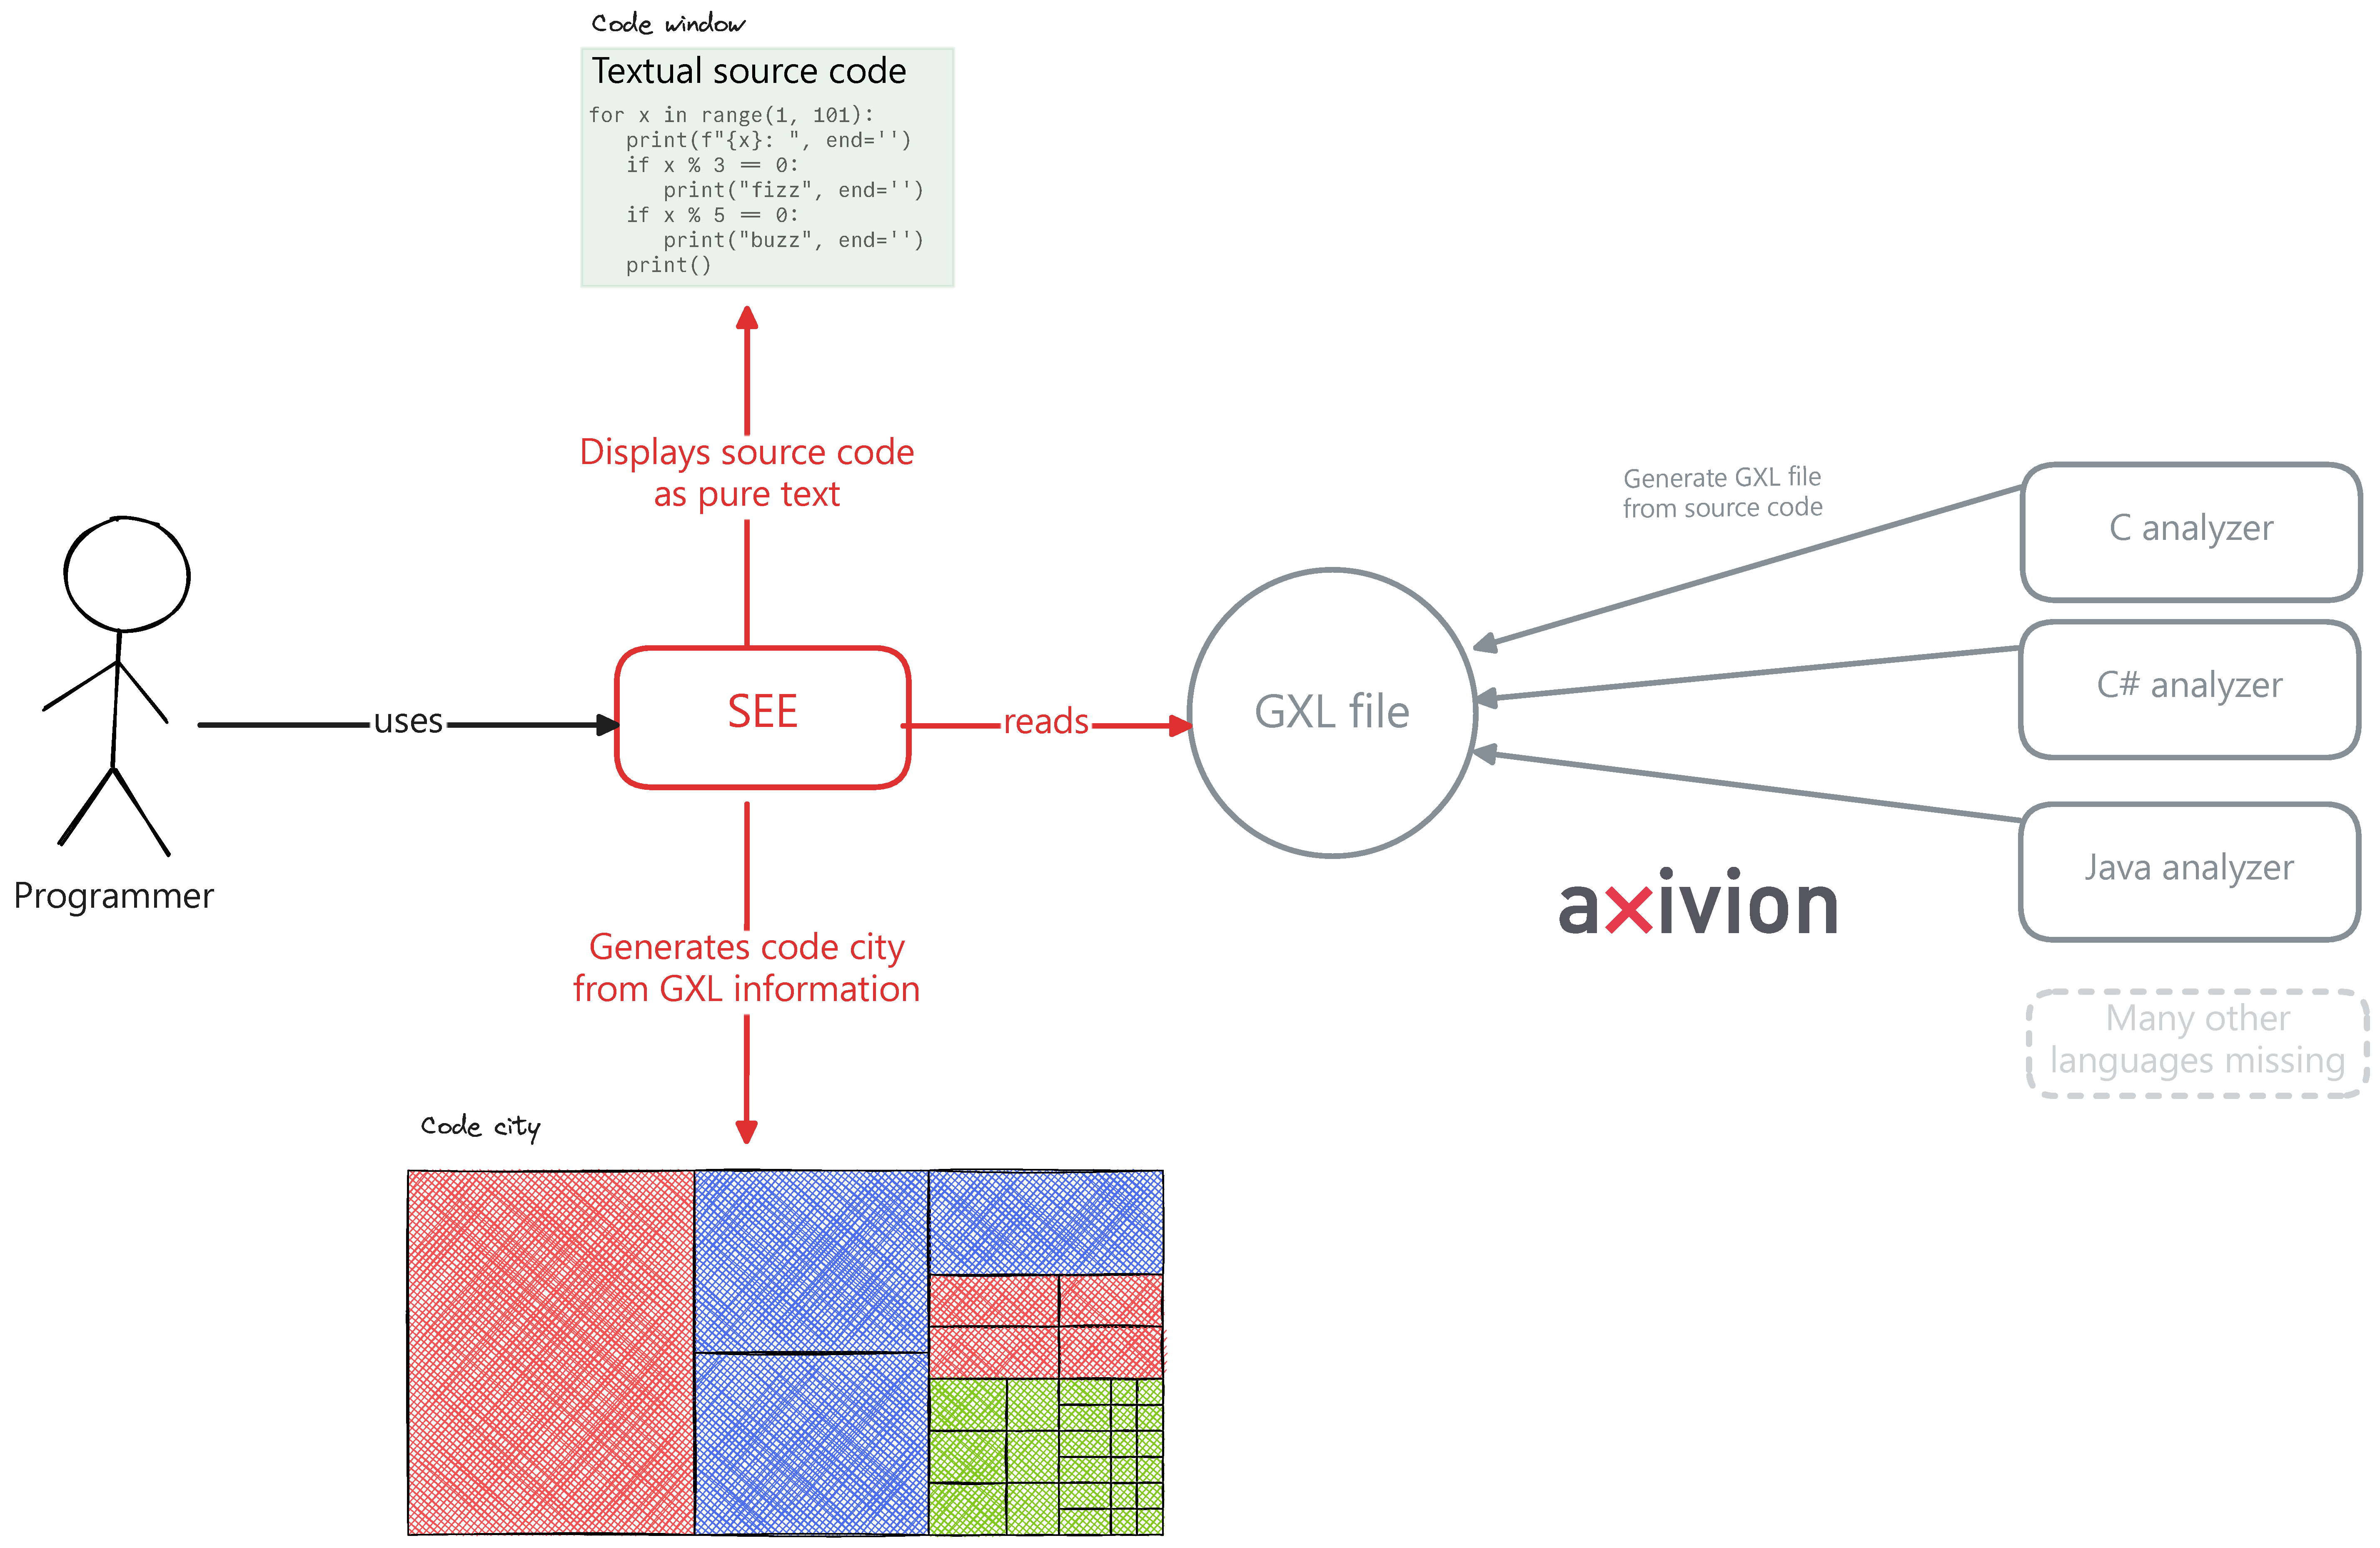
\includegraphics[width=0.95\textwidth]{figures/overview_see_without_lsp}}
    \subcaptionbox{\SEE{} with implemented LSP integration. The language servers on the right are mostly developed by the open-source community.}{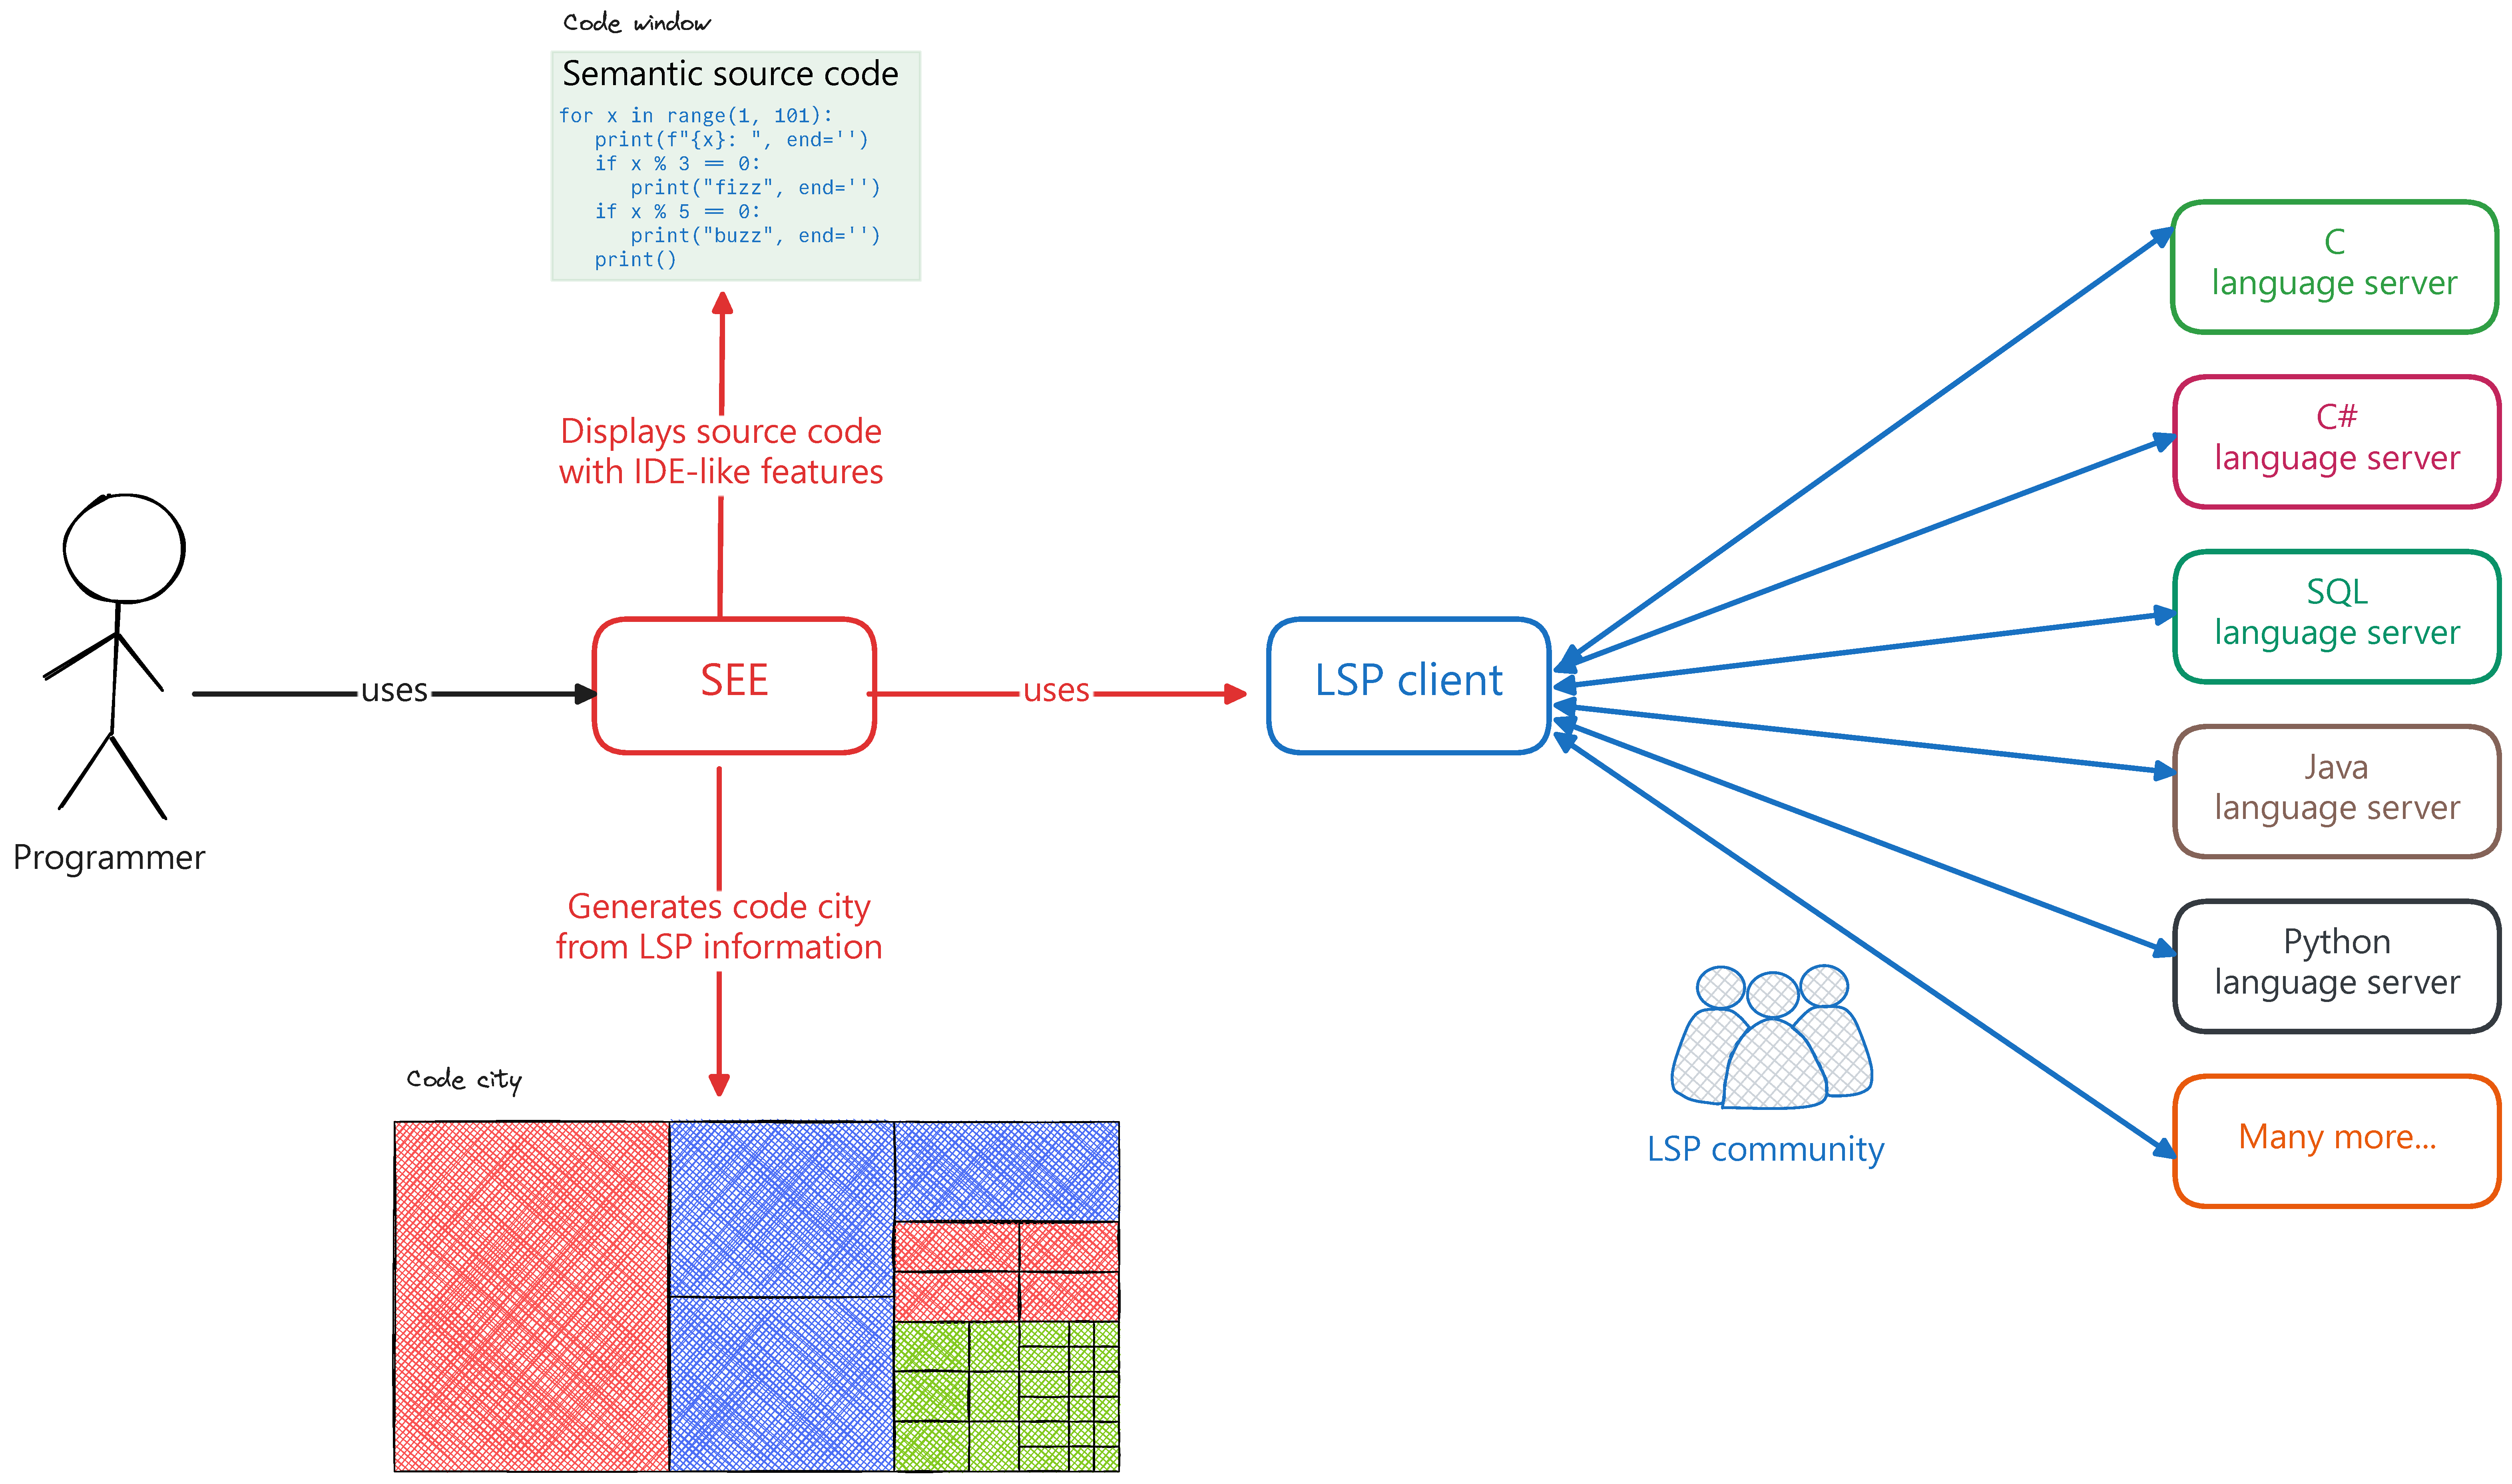
\includegraphics[width=0.95\textwidth]{figures/overview_see_with_lsp}}
  \end{center}
  \caption{A simplified illustration of how \SEE{} currently gains and uses information about software projects, and how the integration of LSP would change that.}\label{fig:seeplan}
\end{figure}

\subsubsection{Generating code cities using LSP}\label{subsubsec:generate}
Before working on the actual code city generation, a required preliminary step is to add an LSP client component to \SEE{}.
As per the LSP specification~\cite{lsp}, this component would then be responsible for both connecting to the Language Server and for managing its lifecycle, that is, starting it and shutting it down.
Additionally, there should be a graphical user interface in \SEE{} (either in-game or in the Unity editor) with which LSP servers can be added, removed, and configured.
Note that it is still the user's responsibility to setup language servers by, for example, installing them via their system's package manager.

The general algorithm of how code cities---or more specifically, their underlying dependency graphs---can be generated from information obtained via LSP is specified\footnote{
  This part is described in such detail because the approach of generating a dependency graph using only LSP information is a new and unorthodox way of using LSP, as it is primarily intended for IDEs and code editors.
} in detail in Algorithm~\ref{alg:generate}.
In that algorithm, we assume that as part of the input, we have a family of LSP functions which are run on the underlying software project.
Accessing an attribute \texttt{y} on an object $x$ returned by an LSP function has the notation $x\texttt{.y}$.
The graphs are formalized as $G = (V, E, a, s, t, \ell)$, with:
\begin{itemize}
  \item $V$ being a set of nodes and $E$ being a set of edges.
  \item $a: (V \times \mathcal{A}_K) \rightharpoonup \mathcal{A}_V$ associating nodes and an attribute name $(\in \mathcal{A}_{K})$ with a value $(\in \mathcal{A}_{V})$. Note that this is a partial function.
  \item $s: E \rightarrow V$ denoting the source node of an edge.
  \item $t: E \rightarrow V$ denoting the target node of an edge.
  \item $\ell: E \rightarrow \Sigma$ providing a label for an edge over some alphabet $\Sigma$ (e.g., to denote its type).
    Also, $\texttt{partOf} \in \Sigma$ such that the subgraph $(V, \{e \in E \mid \ell(e) = \texttt{partOf}\}, a, s, t, \ell)$ is a polytree.
\end{itemize}

\algrenewcommand\alglinenumber[1]{{\footnotesize\textcolor{Gray}{\texttt{#1}}}}
\algrenewcommand\algorithmicrequire{\textbf{Input: }}
\algrenewcommand\algorithmicensure{\textbf{Output: }}

\begin{algorithm}
  \floatname{algorithm}{Algorithm}
  \caption{How code city graphs can be generated from LSP information.}\label{alg:generate}
  \begin{algorithmic}[1]
    \Require  {Family of \textsc{Lsp} functions provided by the Language Server}, {set of documents $D$}
    \Ensure {Graph $G$ representing the underlying software project}
    \Statex
    \State $V, E, a, s, t, \ell \gets \emptyset$ \Comment{Initialize empty graph components.}
    \ForAll{$d \in D$}
      \State $V \gets V \cup \{d\}$ \Comment{Each document becomes a node, with its symbols as children.}
      \ForAll{$s \in \textsc{LspDocumentSymbols}(d)$}
        \State \Call{MakeChild}{\Call{AddSymbolNode}{$s$}, $d$}
      \EndFor
    \EndFor

    \ForAll{$v \in V$}
      \State \Call{ConnectNodeVia}{\textsc{LspGoToDeclaration}, \texttt{Declaration}, v}
      \State \Call{ConnectNodeVia}{\textsc{LspGoToDefinition}, \texttt{Definition}, v}
      \State \Call{ConnectNodeVia}{\textsc{LspGoToTypeDefinition}, \texttt{TypeDefinition}, v}
      \State \Call{ConnectNodeVia}{\textsc{LspGoToImplementation}, \texttt{Implementation}, v}
      \State \Call{ConnectNodeVia}{\textsc{LspReferences}, \texttt{Reference}, v}

      \If{$a(v, \texttt{Type}) = \text{"Method"}$}  
      \Comment{We need to integrate the call hierarchy into the graph.}
        \State $I \gets \Call{LspPrepareCallHierarchy}{a(v, \texttt{SourcePath}), a(v, \texttt{SourceRange})}$
        \LComment{
        \textsc{GetMatchingItem} just returns the item in $I$ with the same name, kind, and location as $v$.
      }
        \State $i \gets \Call{GetMatchingItem}{I, v}$
        \State $R \gets \Call{LspCallHierarchyOutgoingCalls}{i}$
        \LComment{\textsc{GetMatchingNode} returns the node in $V$ with the same name, kind, and location as $r$.}
        \State $V' \gets \{\Call{GetMatchingNode}{r} \mid r \in R\}$
        \ForAll{$v' \in V'$}
          \State $\Call{AddEdge}{v, v', \texttt{OutgoingCall}}$
        \EndFor
        % prepare: receive list of items at position.
        % get item that matches with node.
        % get outgoing call items.
        % get nodes matching those items.
        % create outgoing edge.
      \ElsIf{$a(v, \texttt{Type}) = \text{"Type"}$}
      \Comment{We need to integrate the type hierarchy into the graph.}
        \State $I \gets \Call{LspPrepareTypeHierarchy}{a(v, \texttt{SourcePath}), a(v, \texttt{SourceRange})}$
        \State $i \gets \Call{GetMatchingItem}{I, v}$
        \State $R \gets \Call{LspTypeHierarchySupertypes}{i}$
        \State $V' \gets \{\Call{GetMatchingNode}{r} \mid r \in R\}$
        \ForAll{$v' \in V'$}
          \State $\Call{AddEdge}{v, v', \texttt{Supertype}}$
        \EndFor
        % prepare: receive list of items at position.
        % get item that matches with node.
        % get subtype items.
        % get nodes matching those items.
        % create subtype edge.
      \EndIf{}
    \EndFor


    \State \Return $(V, E, a, s, t, \ell)$

    \Statex
    \algstore{lspcity}
  \end{algorithmic}
\end{algorithm}

% \usepackage{algorithm,algorithmicx,algpseudocode}
\begin{algorithm}
  \begin{algorithmic}[1]
    \algrestore{lspcity}
    \Function{AddSymbolNode}{$s$}
      \State $v \gets \Call{NewNode}{\null}$
      \State $a' \gets \emptyset$
      \State $a'(v, \texttt{SourceName}) \gets s\texttt{.name}$
      \State $a'(v, \texttt{Type}) \gets s\texttt{.kind}$
      \State $a'(v, \texttt{SourcePath}) \gets d$
      \State $a'(v, \texttt{Deprecated}) \gets (\texttt{deprecated} \in s\texttt{.tags})$
      \LComment{Note that \texttt{range} is composed of a \texttt{start} and \texttt{end}, each consisting of a \texttt{line} and a \texttt{column}.}
      \State $a'(v, \texttt{SourceRange}) \gets s\texttt{.range}$
      \LComment{Several other similar attributes omitted here...}
      % \State $a'(v, \texttt{SourceColumn}) \gets s\texttt{.range.start.character}$
      % \State $a'(v, \texttt{SourceLineEnd}) \gets s\texttt{.range.end.line}$
      % \State $a'(v, \texttt{SourceColumnEnd}) \gets s\texttt{.range.end.character}$
      \State $a'(v, \texttt{HoverInfo}) \gets \Call{LspHover}{d, s\texttt{.range}}$
      \If{$a' \nsubseteq a$} \Comment{If node does not already exist...}
        \State $V \gets V \cup \{v\}$
        \Comment{...add it and handle its children.}
        \State $a \gets a \cup a'$
        \ForAll{$s' \in s$\texttt{.children}}
          \State \Call{MakeChild}{\Call{AddSymbolNode}{$s'$}, $v$}
          \Comment{Recurse.}
        \EndFor
      \EndIf
      \State \Return{$v$}
    \EndFunction

    \Statex
    \Function{MakeChild}{$v_c, v_p$}
      \LComment{The \texttt{partOf} edges must induce a tree structure. 
      Hence, if a node already is a part of another node, we must not add another \texttt{partOf} edge.}
      \If{$\exists e \in E: \ell(e) = \texttt{partOf} \land s(e) = v_c$}
        \State \Output{Warning: Hierarchy is cyclic. Some children will be omitted.}
      \Else
        \State $\Call{AddEdge}{v_c, v_p, \texttt{partOf}}$
      \EndIf
    \EndFunction

    \Statex
    \Function{ConnectNodeVia}{$\textsc{LspFun}, \texttt{type}, v$}
    \LComment{Function $\textsc{LspFun}$ only returns locations, so we need to locate the relevant nodes first.}
    \ForAll{$(d, r) \in \Call{LspFun}{a(v, \texttt{SourcePath}), a(v, \texttt{SourceRange})}$}
        \ForAll{$v' \in \Call{FindNodesByLocation}{d, r}$}
        \State $\Call{AddEdge}{v, v', \texttt{type}}$
        \EndFor
      \EndFor
    \EndFunction

    \Statex
    \Function{AddEdge}{$v_s, v_t, l$}
        \State $e' \gets \Call{NewEdge}{\null}$
        \State $E \gets E \cup \{e'\}$
        \State $s(e') \gets v_s$
        \State $t(e') \gets v_t$
        \State $\ell(e') \gets l$
    \EndFunction

    \Statex
    \Function{FindNodesByLocation}{$\texttt{doc}, \texttt{range}$}
    \LComment{We pick the nodes with the most specific range containing the given location.}
    \State $B \gets \{ v \in V \mid a(v, \texttt{SourcePath}) = \texttt{doc} \land \texttt{range.start.line}, \texttt{range.end.line} \in [a(v, \texttt{SourceRange})\texttt{.start.line}, a(v, \texttt{SourceRange})\texttt{.end.line}] \land 
      \texttt{range.start.column} \geq a(v, \texttt{SourceRange})\texttt{.start.column} \land
      \texttt{range.end.column} \leq a(v, \texttt{SourceRange})\texttt{.end.column}
    \}$
    \State {$B \gets \argmin\limits_{v \in B} a(v, \texttt{SourceRange})\texttt{.end.line} - a(v, \texttt{SourceRange})\texttt{.start.line}$}
    \State \Return{$\argmin\limits_{v \in B} a(v, \texttt{SourceRange})\texttt{.end.column} - a(v, \texttt{SourceRange})\texttt{.start.column}$}
    \EndFunction
  \end{algorithmic}
\end{algorithm}



\subsubsection{Integrating LSP into code windows}\label{subsubsec:window}
As mentioned before, code windows, which currently only display the source code without any additional navigational features, should gain "read-only" IDE-like functionality.
Specifically, as listed in \autoref{sec:capabilities}, the following should be supported:
\begin{itemize}
  \item By right clicking on a method and selecting "call hierarchy", a list of incoming and outgoing calls for this method should be displayed.
    Clicking on a call should open the location of that call in the code window.
    \begin{itemize}
      \item Right clicking on a type and selecting "type hierarchy" should work similarly.
    \end{itemize}
  \item Code ranges mentioned by diagnostics should be highlighted, while hovering above such a code range should display details, similar to the already implemented highlighting of code smells detected by the Axivion Suite~\cite{falko}.
  \item Right-clicking on a suitable element and clicking on "Go to declaration" should open a list of declarations, whereas clicking on a declaration should lead to that location being opened in the code window.
    If there is only one declaration, the selection step should be skipped.
    \begin{itemize}
      \item This should work equivalently for "Go to definition/implementation/type definition" and "show references".
    \end{itemize}
  \item Hovering over an item with associated hover information should lead to that information being displayed next to the cursor.
  \item Finally, if the Semantic Tokens capability is supported by the Language Server, syntax highlighting should be implemented using this information.
\end{itemize}

\subsubsection{Extending code city functionality}\label{subsubsec:city}
There is an important difference between the way LSP functionality is integrated into code windows and the way it is integrated into code cities.
For the former, actual JSON-RPC queries are sent to the Language Server whenever an LSP capability is used (as intended by the specification).
However, for code cities, we need not actually do this:
The relevant information for all nodes and edges has already been retrieved as part of Algorithm~\ref{alg:generate} when the code city was generated, and is stored in the form of attributes within the graph elements.
As such---and importantly, because the code city is static---there is no need to introduce the additional overhead of communication with the Language Server here.

Since most of the LSP-provided "read-only" functionality has already been used as part of the code city generation, only the following three features need to be added:
\begin{itemize}
  \item Similar context menu options as for the code windows should be added, such as "show references" or "go to declaration".
    Rather than opening the corresponding location in a code window, the node corresponding to that location should be highlighted in the scene instead.
  \item Code smell icons~\cite{falko} should be displayed above a node for diagnostics scoped to that node.
    Icons should be partitioned based on their severity or tags.
  \item LSP-provided hover information should be displayed when hovering above a node.
\end{itemize}


\subsection{Evaluation}\label{subsec:evaluation}
Finally, the integration of LSP into code cities shall be evaluated via a user study.
Since the integration into the code windows is not a novel approach, this aspect of the implementation will not be evaluated, and I will purely focus on the generated code cities.

My goal is to have at least 10 participants (but ideally, at least 20) take part in the experiment to have a meaningfully representative sample.
In the study, participants will attempt to solve a software engineering task (e.g., understanding a piece of software, or finding out certain information about it) either in \SEE{} or in an LSP-enabled IDE, such as \textit{Visual Studio Code}, or \textit{JetBrains \textsc{IntelliJ}}.
Ideally, participants would be able to do this remotely (both to make it easier to participate and to avoid bias from the Hawthorne effect) by downloading a copy of \SEE{} and the IDE, then following a remote questionnaire.
Aside from measuring task accuracy and time to complete the task, participants will also be given a post-task and/or post-study questionnaire to measure the subjective user experience of \SEE{} versus the IDE.

The research question I seek to answer here is whether code cities are a suitable means to present LSP information to developers as compared to IDEs---specifically, whether code cities are better than, as good as, or worse than IDEs for this purpose on the dimensions of speed, accuracy, and usability.

\section{Schedule}
As of today, \today{}, the implementation has been completed, while the evaluation (and master's thesis itself) still remains to be done.
Below is a rough schedule outlining the remaining steps to be taken, as well as completion dates for finished milestones.
\begin{enumerate}
    \item \textbf{May 1, 2024}: Finished code city generation via LSP as described in \autoref{subsubsec:generate}.
    \item \textbf{June 18, 2024}: Finished extending code city functionality via LSP information as described in \autoref{subsubsec:city}.
    \item \textbf{August 1, 2024}: Finished integrating LSP into code windows as described in \autoref{subsubsec:window} (and thereby finished the implementation part as a whole).
    \item \textbf{August 14, 2024}: Finished preparation of the evaluation (i.e., setting up the user study).
    \item \textbf{September, 2024}: Finished the evaluation as described in \autoref{subsec:evaluation}.
    \item \textbf{October, 2024}: Completed the master's thesis.
      After this date, only smaller details (e.g., formatting improvements) and fixes (e.g., for spelling mistakes) should be applied.
    \item \textbf{November, 2024}: Finished and submitted the master's thesis.
\end{enumerate}

\newpage
\appendix

\section{LSP capabilities}\label{sec:capabilities}

\begin{tabularx}{\textwidth}{@{}lXX@{}}
\toprule
\multicolumn{1}{c}{\textbf{Capability}} & \multicolumn{1}{c}{\textbf{Code Windows}}                        & \multicolumn{1}{c}{\textbf{Code Cities}}                  \\ \midrule
\textit{Call Hierarchy}   & Show incoming/outgoing calls and allow jumping to caller & Generate corresponding edges                    \\
\textit{Diagnostics}                    & Highlight corresponding code ranges and display details on hover & Display code smell icons~\cite[see][]{falko} \\
\textit{References}       & Show references and allow jumping to usage               & Generate corresponding edges                    \\
\textit{Document Symbols} & ---                                                      & Generate corresponding nodes and hierarchy      \\
\textit{Go to Location\footnote{
  This includes the \textit{Go to Declaration, Go to Definition, Go to Implementation,} and \textit{Go to Type Definition} capabilities.
}} & Show locations and allow jumping to them                 & Generate corresponding edges                    \\
\textit{Hover}            & Show hover information when hovering above item          & Show hover information when hovering above node \\
\textit{Semantic Tokens}  & Extended ("semantic") syntax highlighting                & ---                                             \\
\textit{Type Hierarchy}   & Show sub-/supertypes and allow jumping to them           & Generate corresponding edges                   \\\bottomrule
\end{tabularx}


\printbibliography[heading=bibnumbered]

\end{document}
